\documentclass{beamer}
\usepackage{etex}
\usepackage[english]{babel}
\usepackage[utf8]{inputenc}
\usepackage{amsmath}
\usepackage{graphicx}
\usepackage{pgfplots}
\usepackage{caption}
\usepackage{float}
\usepackage{hyperref}
\usepackage{colortbl}
\usepackage{amssymb}
\usepackage{geometry}
\usepackage{booktabs}
\usepackage{etoolbox}
\usepackage{ragged2e}
\usepackage{float}
\usepackage{subcaption}
\usepackage{multirow}
\usepackage{dcolumn}

\newcommand{\etal}{et al.}
\usepackage[figurename=]{caption}

\usetheme{Boadilla}
\setbeamersize{text margin left=0.5cm,text margin right=0.5cm}
\newcommand\FontDetalleTecnico{\fontsize{8}{9.2}\selectfont}
\tikzset{
  font={\fontsize{7pt}{8}\selectfont}
  }

%change footer format
\makeatother
\setbeamertemplate{footline} 
{
  \leavevmode%
  \hbox{%
  \begin{beamercolorbox}[wd=.3\paperwidth,ht=2.25ex,dp=1ex,center]{author in head/foot}%
    \usebeamerfont{author in head/foot}\insertshortinstitute
  \end{beamercolorbox}%
  \begin{beamercolorbox}[wd=.6\paperwidth,ht=2.25ex,dp=1ex,center]{title in head/foot}%
    \usebeamerfont{title in head/foot}\insertsection
  \end{beamercolorbox}%
  \begin{beamercolorbox}[wd=.1\paperwidth,ht=2.25ex,dp=1ex,center]{date in head/foot}%
    \insertframenumber{} / \inserttotalframenumber\hspace*{1ex}
  \end{beamercolorbox}}%
  \vskip0pt%
}
\makeatletter
%add table of content before each section
\AtBeginSection[]
{
  \begin{frame}
    \frametitle{Contents}
    \footnotesize{
    \tableofcontents[currentsection]
    }
  \end{frame}
}
\setbeamerfont{footnote}{size=\tiny}
%justify itemize
\makeatletter
\renewcommand{\itemize}[1][]{%
  \beamer@ifempty{#1}{}{\def\beamer@defaultospec{#1}}%
  \ifnum \@itemdepth >2\relax\@toodeep\else
    \advance\@itemdepth\@ne
    \beamer@computepref\@itemdepth% sets \beameritemnestingprefix
    \usebeamerfont{itemize/enumerate \beameritemnestingprefix body}%
    \usebeamercolor[fg]{itemize/enumerate \beameritemnestingprefix body}%
    \usebeamertemplate{itemize/enumerate \beameritemnestingprefix body begin}%
    \list
      {\usebeamertemplate{itemize \beameritemnestingprefix item}}
      {\def\makelabel##1{%
          {%
            \hss\llap{{%
                \usebeamerfont*{itemize \beameritemnestingprefix item}%
                \usebeamercolor[fg]{itemize \beameritemnestingprefix item}##1}}%
          }%
        }%
      }
  \fi%
  \beamer@cramped%
  \justifying% NEW
  %\raggedright% ORIGINAL
  \beamer@firstlineitemizeunskip%
}
\makeatother


% LECTURE INFORMATION
\title{ML week slides template}
\institute{EEPP IIS-UNSAAC}

\author{Lecturer name\\
        lecturer mail}

\date{\today}


% SLIDES EXAMPLE STARTS HERE 
\begin{document}
%cover of slides
\frame{\titlepage}
%table of contents
\begin{frame}
    \frametitle{Contenido}
    \footnotesize{
    \tableofcontents
    }
\end{frame}

%start editing here
\section{Ejemplo de sección 1} % ----------------------------------
\subsection{Ejemplo de subsección 1}
\begin{frame} 
   \frametitle{Ejemplo de título 1}
   \begin{itemize}
   \item Ejemplo de item 1.
   \item Ejemplo de item 2.
   \item Below an example of figure and reference.
   \end{itemize}
   \begin{figure}[!htb]
        \centering
        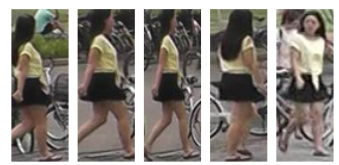
\includegraphics[width=0.6\textwidth]{figs/re-id1.png}
        \caption{image caption  \textbf{Source:} Karanam \etal\footnote{S. Karanam, M. Gou, Z. Wu, A. Rates-Borras, O. Camps, and R. J. Radke. A Systematic Evaluation and Benchmark for Person Re-Identification: Features, Metrics, and Datasets. arXiv preprint arXiv:1605.09653, 2016.}}
    \end{figure}
\end{frame}

\subsection{Ejemplo de subsección 2}
\begin{frame}
    \frametitle{Ejemplo de bloque}
    \begin{block}{}
    Este es un bloque
    \end{block}
\end{frame}

\section{Ejemplo de sección 2} % ----------------------------------
\subsection{Ejemplo de subsección 1}
\begin{frame}
    \frametitle{Ejemplo de tabla}
    \small
    \begin{table}[!htb]
    \setlength{\tabcolsep}{1.1mm}
    \renewcommand{\arraystretch}{1.1}
    \centering
    \footnotesize % 
    \begin{tabular}{lcrr}
    \toprule
    \textbf{Data Set}  & \textbf{Year} & \#\textbf{People} & \#\textbf{BBox} \\
    \midrule
    PRID2011    & 2011 & 934   & 24,541 \\
    iLIDS-VID   & 2014 & 300   & 42,495 \\
    MARS        & 2016 & 1,261 & 1,192 \\
    \bottomrule
    \end{tabular}
    \end{table}
\end{frame}

\begin{frame}
    \Huge Gracias!
\end{frame}

\end{document}

